

\chapter{Design}
\label{ch:design}
The design of the project consist of three individual sections, that are then combined to produce a resulting application. These are: The Emulator \ref{sec:emulator}, Visualisation \ref{sec:visualisation} and the Module System \ref{sec:module}. The module system was not originally a section, but was considered later on and then designed to allow for RISC-V extensions to be included. The use of "extension" and "module" may be confused within this section, however it should be identified as: "We create a module that encapsulates the logic of a RISC-V extension".

This approach was chosen to allow for a consistent flow of development, with the Emulator being core to allow the visualisation system to know what to simulate, thus the emulator must be completed first, and then the visualisation built separately and then combined onto of the emulator. The module system can then be attached on later once it was designed. 

Together these 3 sections encapsulate the entire project and its complete functionality, and the inclusion of the Module system allows us to satisfy requirements \ref{req:md} and \ref{req:fp} to include the Multiply and Divide, and Single Precision Floating Point Module. And, with these 3 sections being created completely from scratch it provides the flexibility to independently design and create each, and then combine them later on when required, allowing for a detached design and implementation process.

\begin{figure}[h]
    \centering
    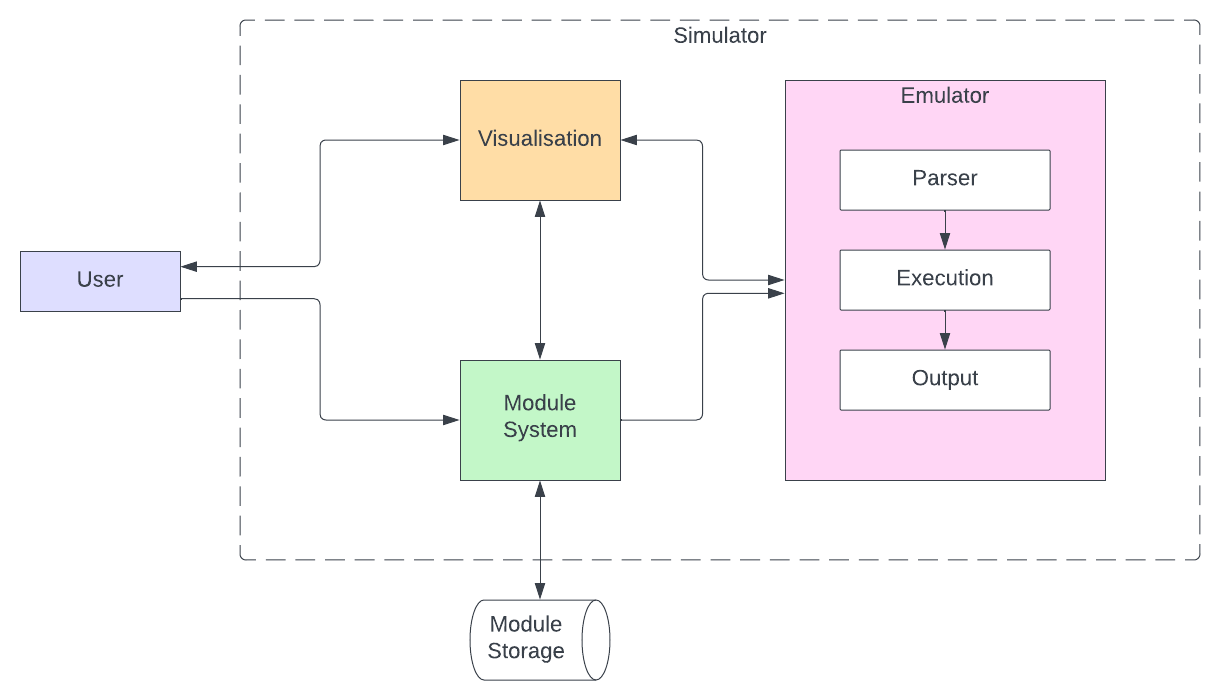
\includegraphics[width=0.95\linewidth]{dissertation/DATA/sys architecture.png}
    \caption{Overall System Architecture}
    \label{fig:sys_architecture}
\end{figure}

In the system architecture diagram in Figure \ref{fig:sys_architecture} we provide an outline of how the 3 sections integrate within the simulator. A user will directly interact with the visualisation layer, in turn the visualisation layer interacts directly with the emulator and module system to provide functionality. This approach was decided upon as the end user should never directly interact with the emulator as this avoids the simulation aspect, and the user should have limited access to the module system to enable, disable, load and unload modules as they require without having to worry about how this impacts the rest of the visualisation or emulator.

Within the system architecture diagram "Module Storage" is provided. This will exist on the users physical machine to store loaded modules to avoid loosing functionality over application restarts.

It is important to consider how a user may interact with the system in everyday use. The user sequence diagram in Figure \ref{fig:user_sequence} describes a typical user flow. The flow covers how a user may start by launching the application and entering a RISC-V program. By hitting "Run" the code is either accepted via a successful parse or rejected and a error is returned to the user. This may repeat several times, until a successful parse occurs. When this happens the program is executed line per line with animations playing out sequentially. After the user decides to manage their modules via the module popup, enabling and disabling the listed modules with a confirmation being shown after each change.

\begin{figure}[h]
    \centering
    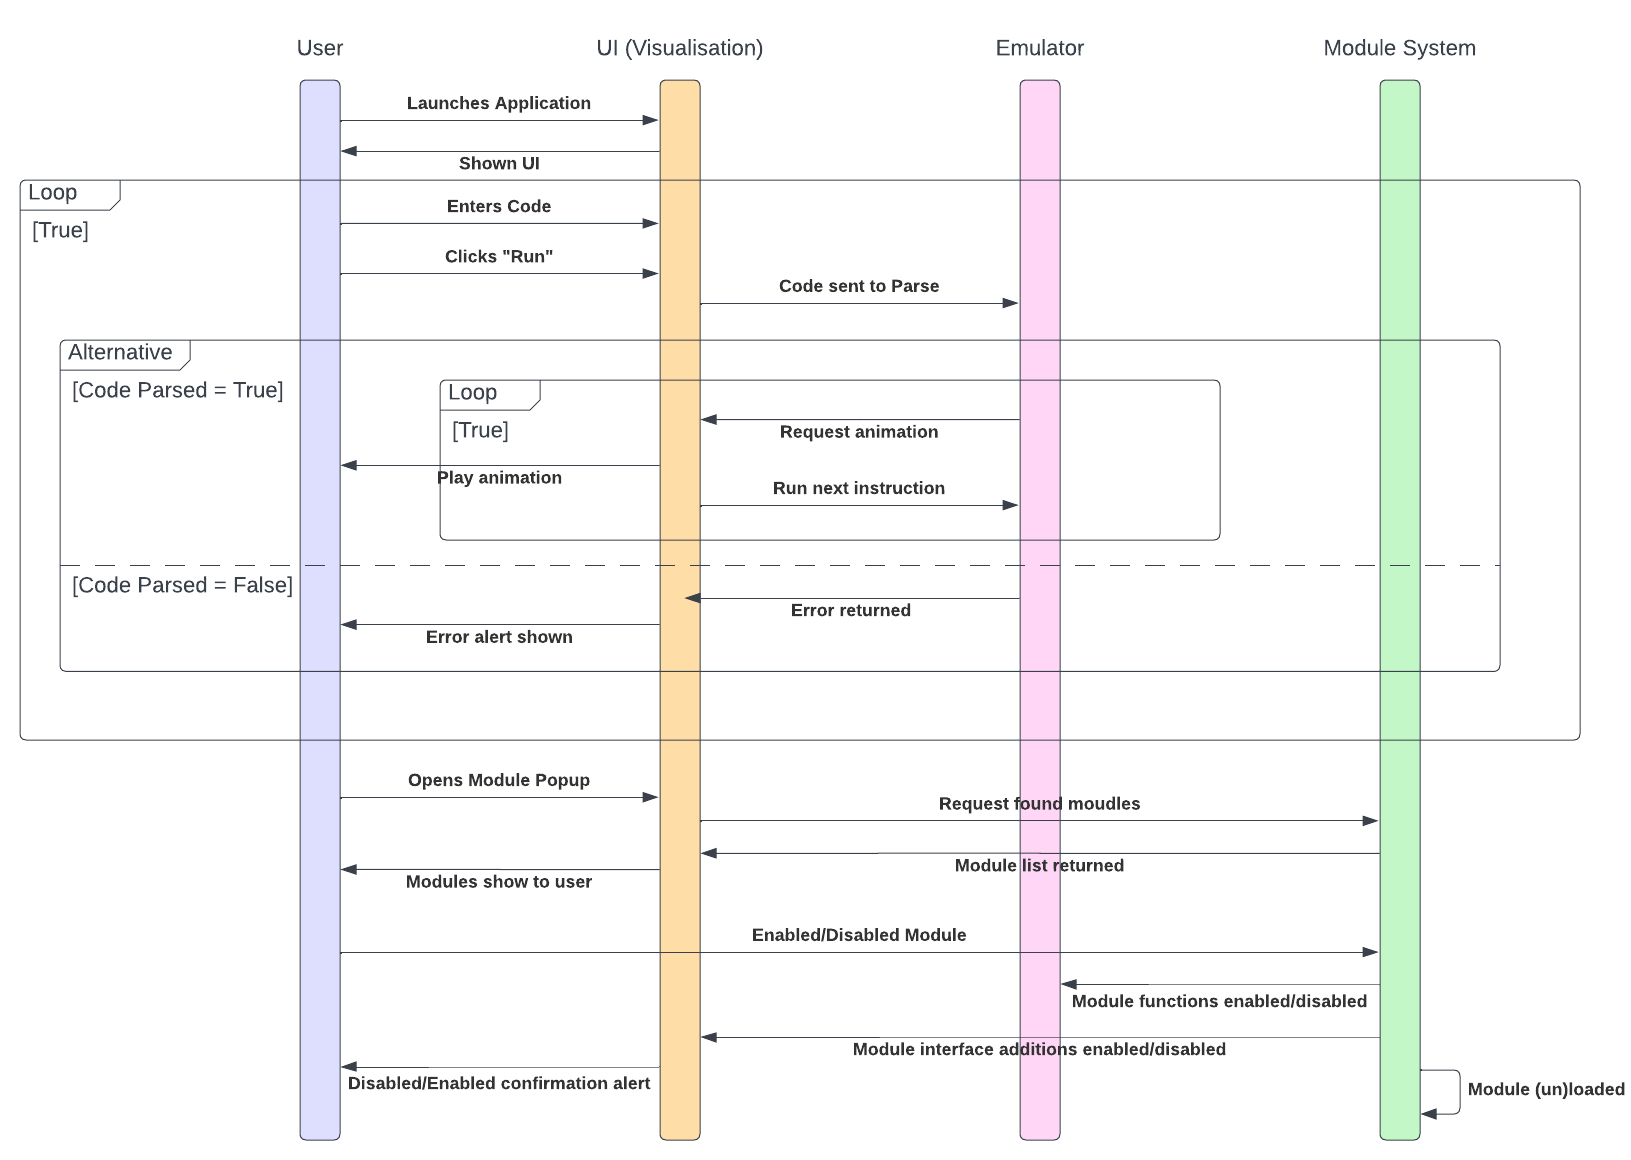
\includegraphics[width=0.95\linewidth]{dissertation/DATA/sequence diagram.png}
    \caption{Example user sequence diagram}
    \label{fig:user_sequence}
\end{figure}

\section{Emulator}\label{sec:emulator}
The emulator is designed to mock the RISC-V architecture closely, whilst also being simple and efficient. In the overall system architecture diagram in figure \ref{fig:sys_architecture} the emulator is denoted as flowing between 3 high level ideas: "Parser", "Execution" and "Output". These are not rigid names, but allow us to comprise a high level overview of the entire emulator with each being discussed below:

\subsection{Parser}\label{sec:parser}
In order for any code to be emulated it must be parsed first. The design for the parser must be simple and efficient, providing suitable error feedback when required.

The parser is designed to consume the inputted user program line-by-line. Each line is expected to conform to a valid instruction with a set amount of operands. For example the following valid ADDI instruction will read register x1, add 3 to it and then write the result back to register x1:\\\\
\verb|ADDI x1, x1, 3|
\\\\
The parser should first identify the instruction name, and then identify the respective operands that the instruction should expect, including how many and of what type each. This can be performed by linearly consuming each inputted operand and checking it conforms to the expected type, whilst pre-checking that there aren't more or less operands than expected, rejecting if anything is invalid, throwing an exception if so. If an instruction is valid, it should be completely consumed and converted into an intermediary instruction format for use later.

\begin{figure}[H]
    \centering
    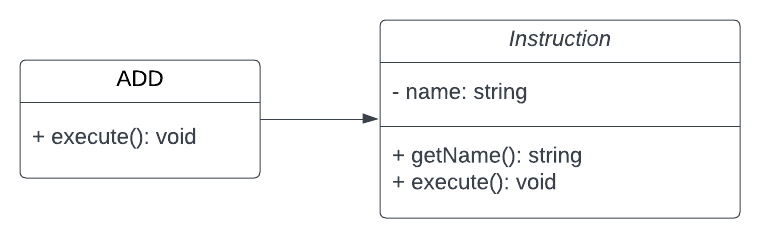
\includegraphics[width=0.95\linewidth]{dissertation/DATA/instr_abstract_uml.png}
    \caption{Basic UML diagram of the Abstract instruction class}
    \label{fig:instr_abstract_uml}
\end{figure}

Figure \ref{fig:instr_abstract_uml} presents this intermediary form. This abstract \texttt{Instruction} class will encapsulate each individual instructions logic, with every instruction extending and overriding the \verb|execute()| method. Figure \ref{fig:instr_abstract_uml} shows an example of an ADD instruction being implemented.

Each individual implementation should be stored centrally and referenced by name such that it may be called later for execution with its parsed operands stored separately such that each instruction may be reused with different operand combinations.


\subsection{Execution}
Execution encapsulates the internal design of the system including the Registers, Memory and how they integrate. There needs to be a consideration first on how both will store a 32 bit binary value. This could simply be a string of of 32$\times$1's and 0's or the based integer type in Java. However the use of a custom \texttt{Binary} object \ref{fig:bin_regmem_uml} would seem more logical to provide consistency between the Register and Memory, with simple functions to both read and write as Binary, Denary and Hex.

The emulation requires a representation of the 32 base registers, with the ability to reference them by not only their name. but also their respective Application Binary Interface (ABI) name as well \cite{riscvinternational_2014_calling}(page 3) which is an alternate name denoting specific usage or idea placement of data. 

A list might work nicely here, allowing direct addressing from 0-31 for the base 31 registers, however if a user addressed via their ABI name we would have to linearly search every register to check its ABI name which is inefficient. Thus a map suites the problem better, with the ability to directly map both the numerical name and ABI name to each register with the ability to read and write via these names as seen in Figure \ref{fig:bin_regmem_uml}, and providing a O(1) lookup time as a additional benefit.

Unlike registers, memory needs to be addressable by its 4 byte aligned location, and thus we could opt for two methods of referencing:
\begin{enumerate}
    \item Use a list and take modulo 4 of addressed to get the relative index in the list for each memory value.
    \item Use a map to store the location as a key, with the memory value as the value, avoiding extra computation to calculate locations.
\end{enumerate}
Both are valid options. However, option 2 provides the benefit of a O(1) lookup time, compared to O(n) for a list, and seeing as the memory may become infinitely large with a complex emulation, option 2 suffices as the better choice.

\begin{figure}[H]
    \centering
    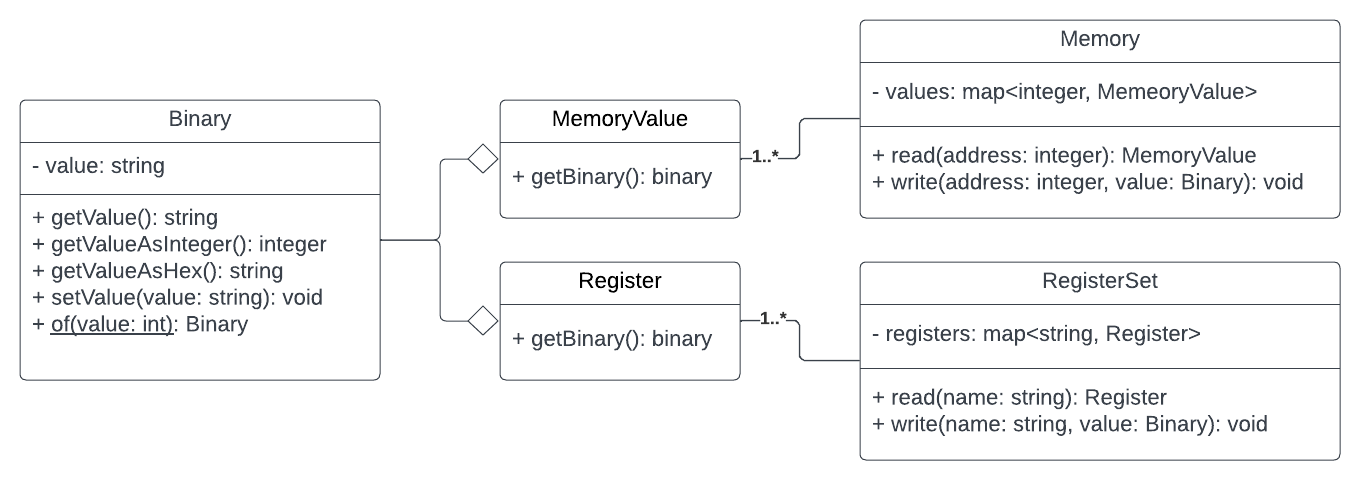
\includegraphics[width=\linewidth]{dissertation/DATA/bin_regmem_uml.png}
    \caption{Binary, Memory and Register UML Diagram}
    \label{fig:bin_regmem_uml}
\end{figure}

\subsection{Output}
Our output design simply come in the form of the handshake it will have with the visualisation section. The Emulator itself should only output the end result, parse errors and signals for animations to take place.

Each should be simple to differentiate, most likely with parse errors being raised as an error by Java that can be caught and passed to the visualisation to be displayed. The end output being printed to the terminal during development and for debugging, and animation signals being preemptively stubbed in code, to be hooked into later by the visualisation system.






\section{Visualisation}\label{sec:visualisation}
The visualisation of the emulation is a large part of the project, with the overall simulation relying heavily on a well designed \ac{UI}, thus the design of the \ac{UI} has been heavily considered to ensure an appropriate interface that presents the right amount of information without being too simple nor too complicated.

\begin{figure}[H]
    \centering
    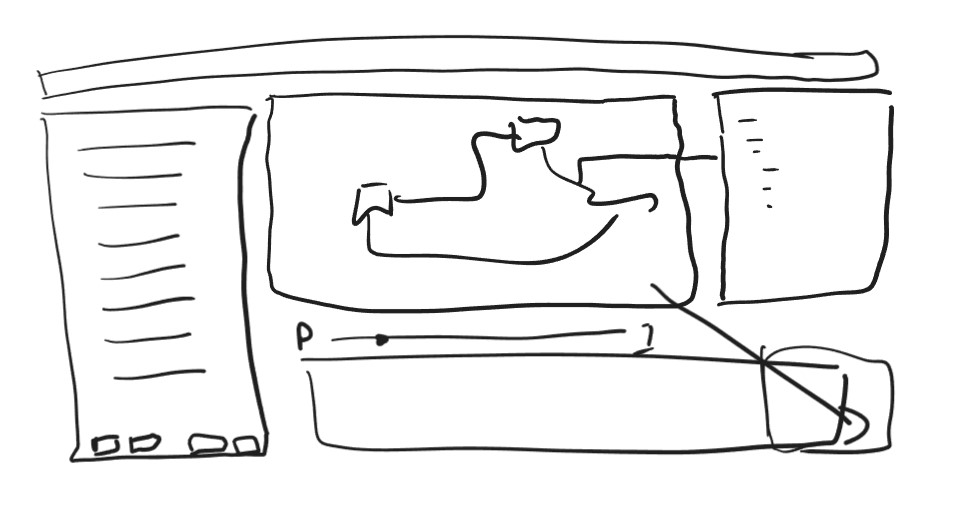
\includegraphics[width=\linewidth]{dissertation/DATA/early_design.jpg}
    \caption{Original hand drawn UI design}
    \label{fig:early_ui_design}
\end{figure}

Our first \ac{UI} design (Figure \ref{fig:early_ui_design}) was designed to be simple, and loosely based on the design of LittleManComputer (Figure \ref{fig:lmc}) and Emulsiv (Figure \ref{fig:emulsiv}) as discussed in Section \ref{sec:lmc} and \ref{sec:emulsiv} respectively. 
The design places the code editor on the left, the main visualisation area in the centre, registers on the right, memory along the bottom and a menu bar stretching the top. These positions were specifically chosen based on the constraint of element sizing:
\begin{itemize}
    \item The code editor requires a large vertical space to hold many lines of code, but a relatively short horizontal width, due to the average instruction being relatively short.
    \item The animation/visualisation area was given the most space as this is the main focus point of the application, and thus being dead centre is the most appropriate location within the \ac{UI}.
    \item Registers, much like the code editor require a small horizontal space to display their value, but 32 of them need to be on display at any given time, thus a large horizontal space allows for this with minimal scrolling on smaller screens.
    \item Memory also requires limited horizontal space, however, unlike registers, it starts of empty for every execution, and may not be used in any given execution, thus designating it to the bottom to fill waste space is more appropriate. Should the memory fill up, the user may scroll through it to see all the values at any given time.
\end{itemize}

Other elements have also been positioned for their own respective reasons irrespective of size constraints:
\begin{itemize}
    \item The menu bar stretches along the top to conform with expected user patterns and expectations, with users commonly expecting it at the top of the application, thus placing it elsewhere would of been unprofessional.
    \item The Settings and Module sections are popups, that display in the middle of the screen. This conforms with user expectations and grabs attention to the popup without having to search for it on screen. It also provides the option to be moved based on the users need, whilst hiding secondary content that is important to the core simulation.
\end{itemize}

As-well as the overall \ac{UI} design, a simple yet intuitive layout needed to be created to visualise the internal data movement around the processor components (\ac{ALU}, \ac{CU}, \ac{IR}, \ac{ID}, Instruction Memory, Registers and Memory). The original design of this can be seen below in Figure \ref{fig:early_animation_design} with, Control Unit designs in Figure \ref{fig:early_cu_design}.

\begin{figure}[H]
    \centering
    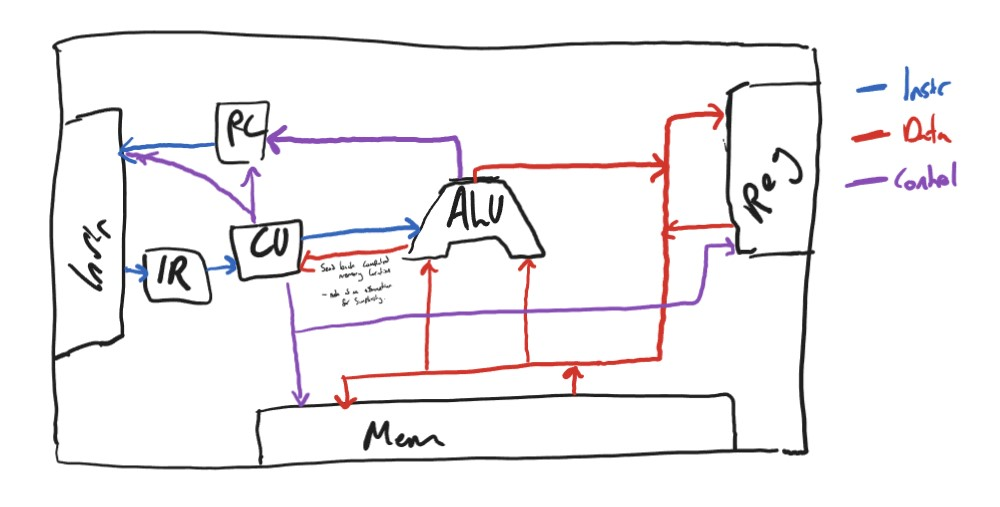
\includegraphics[width=\linewidth]{dissertation/DATA/animation_layout.jpg}
    \caption{Original animation area design}
    \label{fig:early_animation_design}
\end{figure}

\begin{figure}[H]
    \centering
    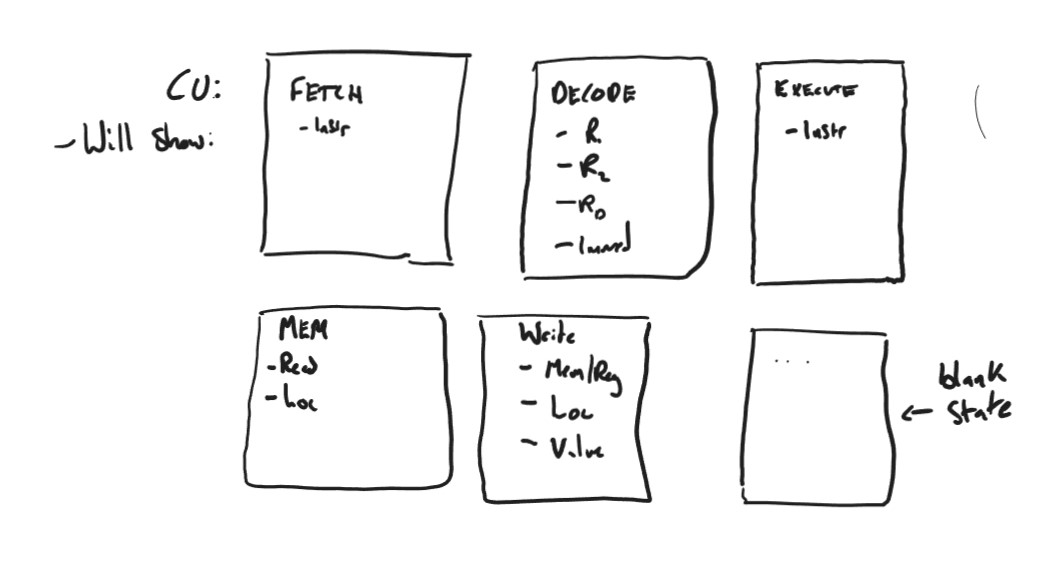
\includegraphics[width=\linewidth]{dissertation/DATA/control_unit.jpg}
    \caption{Original Control Unit design}
    \label{fig:early_cu_design}
\end{figure}

Figure \ref{fig:early_animation_design} displays the concept of the animation area, with components being connected by coloured wires, with blue, red and black representing the transfer of Instructions, Data and Control signals respectively. Allocating larger boxes to side elements that will correspond to the respective \ac{UI} elements on the wider interface.

The \ac{CU} in Figure \ref{fig:early_animation_design} is just displayed as a simple box, however it is intended that it will display mroe data to convey what the emulator is doing, for example what stage is currently operating and some information associated with the stage. Examples of this more detailed design can be seen in Figure \ref{fig:early_cu_design}.

These base designs allowed us to then revise and redesign to improve aspects. During revisions we decided to consider Nielsen's Usability Heuristics \cite{nielsen_2020_10} as covered in section \ref{sec:nielson}. Within this, our design failed 2 principles being 1 and 8 relating to visibility of system  status and aesthetic and minimalist design.

The design failed these due to our choice to redesign to include colour within our interface to help differentiate the animation components. This lead to the used of colours such as red and green which colourblind users are unable to differentiate between, instead appearing as a murky brown. To prevent this issue whilst also maintaining this newer design we switched to using grayscale. This eliminated the issue whilst still providing a way for colourblind users to easily differentiate between processor components and thus making the visability of the system better available to all.

A further design issue was a choice of background colour, which a original change to use a gray background instead of white, going with a darkish gray. However, this produced a low contrast ratio between the background and other element which may prove hard for visually impaired users to see as-well as increasing eye strain. The Web Accessibility Initiative \cite{webaccessibilityinitiativew3_2022_understanding} denotes a minimum contrast ration of 4.5:1, which our original design of gray on gray doesn't provide. Upon further redesigning we switched this dark gray for a much lighter gray, which in turn greatly increased the contrast ratio to an acceptable level.

An overview of the above changes and a few extra are listed below:
\begin{enumerate}
    \item Lightening of the background to increase the contrast ration to an acceptable level,
    \item Convert the red, green and blue boxes to grayscale to alleviate the issue for colourblind users,
    \item Gray boxes were switched to purple to increase contrast.
\end{enumerate}

With all these consideration taken into account the final design was complete, with physical mock up in Figure \ref{fig:final_implemented_design}. (Please note this image has been taken from our implemented design due to the designed version being lost)

\begin{figure}[H]
    \centering
    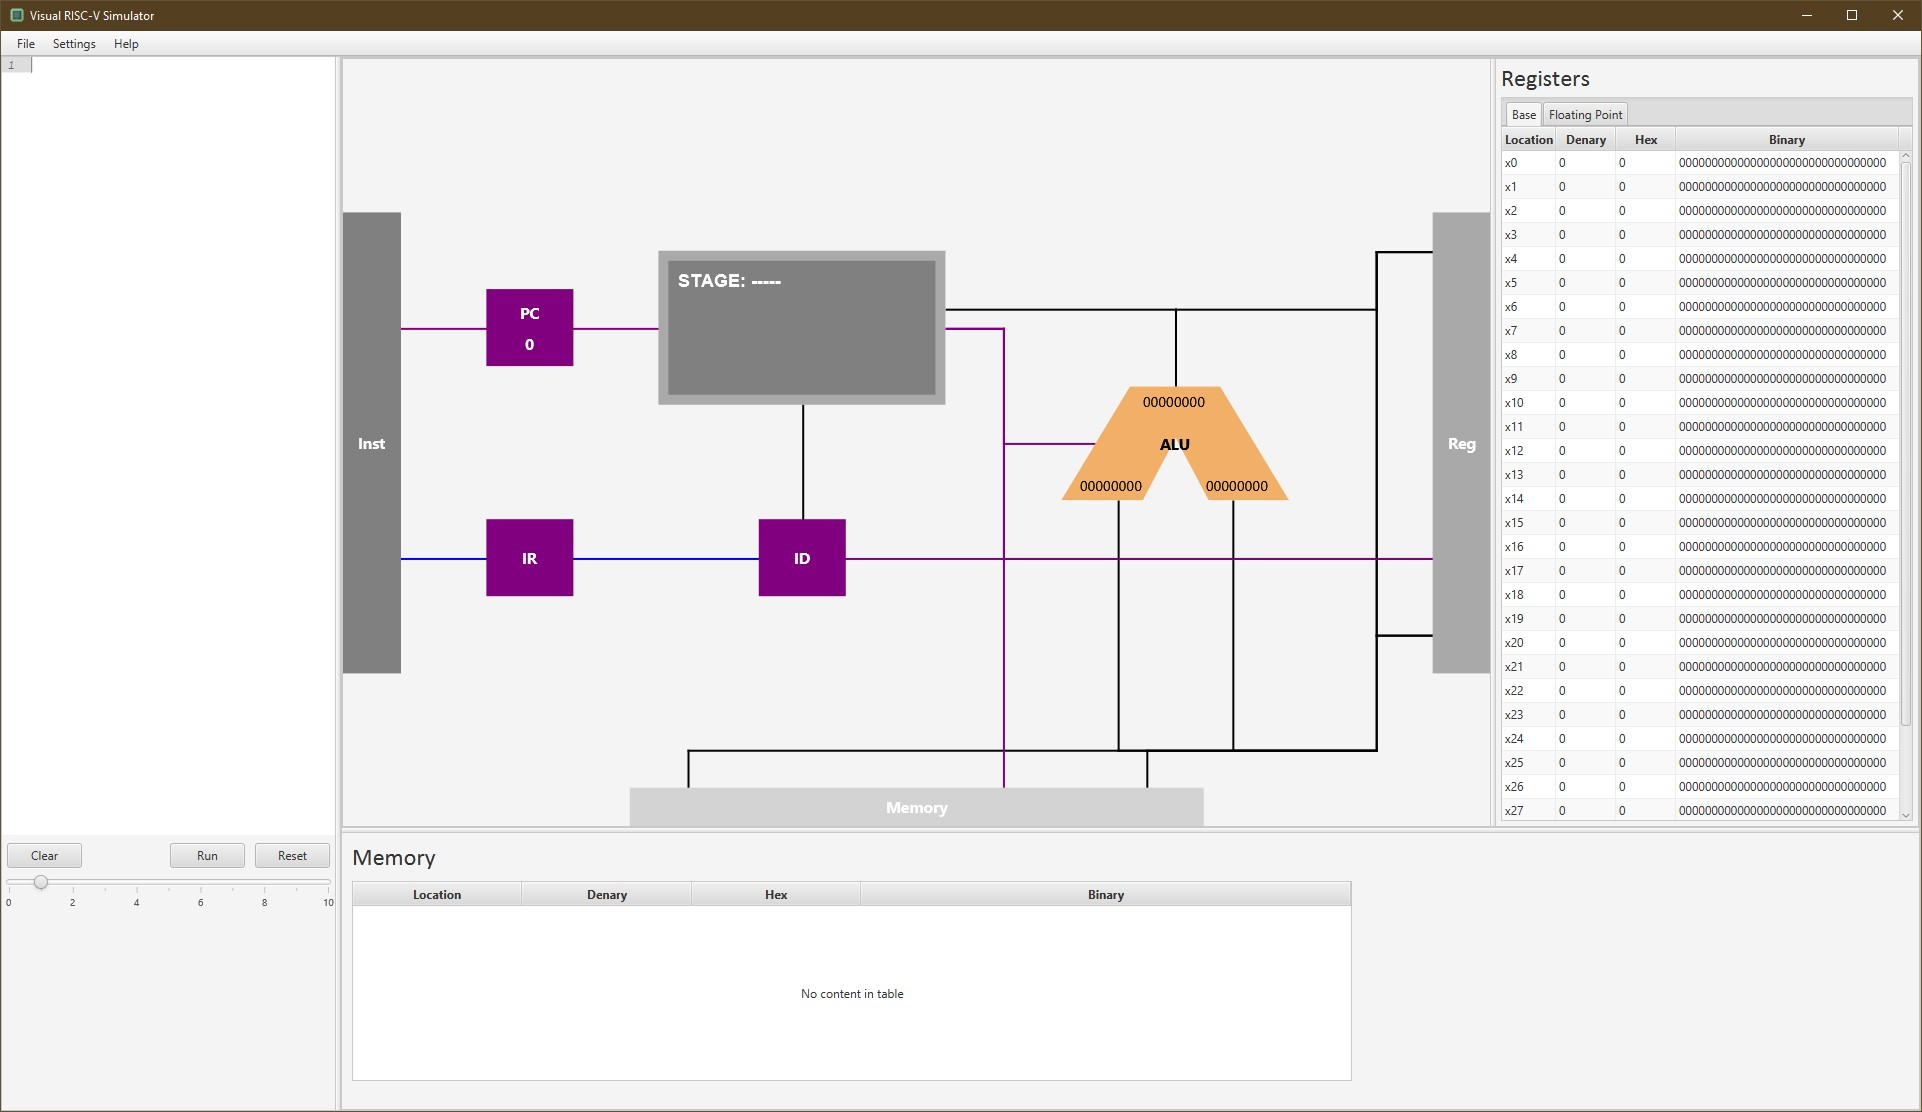
\includegraphics[width=0.9\linewidth]{dissertation/DATA/final_design.jpg}
    \caption{Final full UI design}
    \label{fig:final_implemented_design}
\end{figure}

This final design allows us to follows Nielsen's principles \cite{nielsen_2020_10}, with a simple and minimalist design, with only whats required on screen, and further principle 4, keeping our layout and design consistent across the entire application.





\section{Module System}\label{sec:module}
The applications module system is designed to be convenient and intuitive to use. As mentioned at the start of the design section, modules are implementations of RISC-V extensions and were a later addition that was designed around the emulator. But, could be easily designed in thanks to our simple emulator design, with the ability to directly add new instruction into our map design and reference them via their respective names.

\begin{figure}[H]
    \centering
    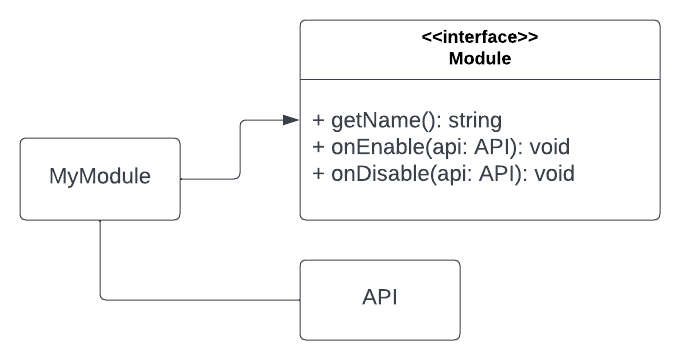
\includegraphics[width=0.9\linewidth]{dissertation/DATA/module uml.png}
    \caption{Module System UML Diagram}
    \label{fig:module_uml}
\end{figure}

Modules are designed to implement a simple module interface (Figure \ref{fig:module_uml}). With the system designed to be able to find and load modules, and then enable and disable the mas required. Modules them self are designed to allow for quick creation to allow the implementation of custom logic, with an enable and disable method providing an API instance discussed below.

This API instance is designed to be simple to allow modules to access the core of the emulator to allow the addition of exra instructions and logic, whilst restricting access to internal systems that shouldn't be modified. 

The overarching system managing individual modules was also designed to be simple, with an option to quickly enable and disable modules, aswell as a simple interface to load and remove modules.

Figure \ref{fig:module_popup} shows an example of the module popup, which will allow users to manage there modules, aswell as enable and disable them.

\begin{figure}[H]
    \centering
    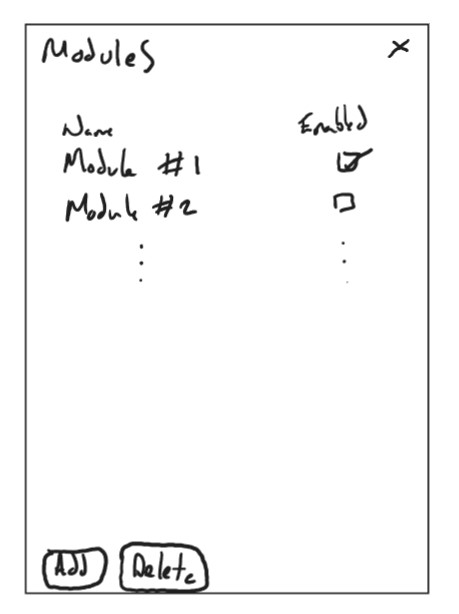
\includegraphics[width=0.7\linewidth]{dissertation/DATA/module design.jpg}
    \caption{Module popup design}
    \label{fig:module_popup}
\end{figure}


